\begin{figure}[htbp]\centering
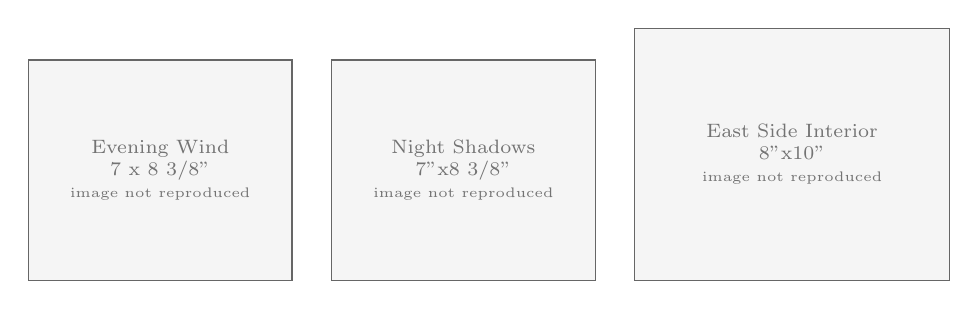
\begin{tikzpicture}
\draw[fill=black!4,draw=black!60,line width=0.5pt] (0,0) rectangle (3.35,2.8000000000000003);
\node[align=center,text=black!55,font=\scriptsize] at (1.675,1.4000000000000001) {Evening Wind\\7 x 8 3/8"\\\tiny image not reproduced};
\draw[fill=black!4,draw=black!60,line width=0.5pt] (3.85,0) rectangle (7.2,2.8000000000000003);
\node[align=center,text=black!55,font=\scriptsize] at (5.525,1.4000000000000001) {Night Shadows\\7"x8 3/8"\\\tiny image not reproduced};
\draw[fill=black!4,draw=black!60,line width=0.5pt] (7.7,0) rectangle (11.7,3.2);
\node[align=center,text=black!55,font=\scriptsize] at (9.7,1.6) {East Side Interior\\8"x10"\\\tiny image not reproduced};
\end{tikzpicture}
\caption{\textbf{Evening Wind}, etching, 1921, 7 x 8 3/8" as the leaf writes it (Book I, leaf 2, ref 16853). The Metropolitan Museum of Art, 25.31.7: \url{https://www.metmuseum.org/art/collection/search/366211}. \textbf{Night Shadows}, etching, 1921, 7"x8 3/8" as the leaf writes it (Book I, leaf 6, ref 16548). The Metropolitan Museum of Art, 25.31.2: \url{https://www.metmuseum.org/art/collection/search/366206}. \textbf{East Side Interior}, etching, 1922, 8"x10" as the leaf writes it (Book I, leaf 8, ref 17539). The Metropolitan Museum of Art, 25.31.1: \url{https://www.metmuseum.org/art/collection/search/366204}. Scale: ten inches to four centimetres, four times the scale of the canvases in the other figures. The frames are drawn to the proportions of the size in Edward Hopper's hand; the images are not reproduced here and can be seen at the museums' own pages. Drawn by Claude Fable~5.1, 13 September 2026, from the transcriptions and \texttt{works.json} (2026-09-13).}\label{fig:etchings}
\end{figure}
